%- block legend
Nada como uma agradável noite com seus amigos na sua casa comendo uma pizza
enquanto assistem seu \textit{anime} favorito!

Opa, a pizza chegou! Como o grupo tem 4 pessoas ao todo, você decidiu cortar a
pizza em 4 pedaços. Você fez um corte horizontal e outro corte vertical, de tal
forma que os cortes intersectam em um ponto $P$ na pizza.

Oh não! Você acabou de perceber que os 4 pedaços podem ter ficado de tamanho
diferentes! Dados o raio da pizza e a coordenada do ponto $P$, determine a área
dos 4 pedaços obtidos.

%- endblock

%- block input
A entrada contém uma linha com três inteiros $R$, $X$ e $Y$
($1 \leq R \leq 30, \sqrt{X^2 + Y^2} < R$), o raio da pizza e as coordenadas do ponto
$P$, respectivamente. Considere que a pizza está centrada na origem (isto é, seu
centro é o ponto $(0,0)$).

%- endblock

%- block output
Imprima uma linha com quatro valores $A_1$, $A_2$, $A_3$ e $A_4$ indicando a área de cada
pedaço da pizza, arredondadas com três casas decimais. Imprima os valores em
ordem não-decrescente (isto é, de forma que $A_1 \leq A_2 \leq A_3 \leq A_4$).
%- endblock

%- block notes
A figura abaixo representa o primeiro exemplo de entrada:
\begin{center}
    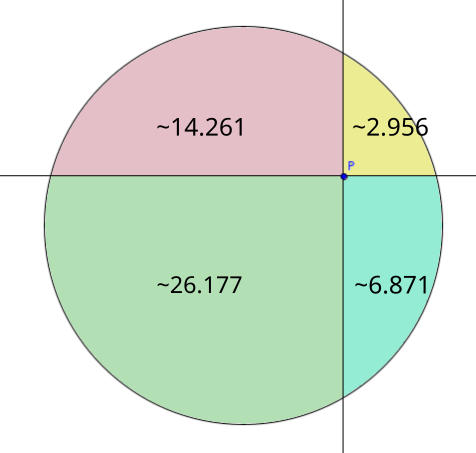
\includegraphics[scale=1.25]{pizza.png}
\end{center}
%- endblock

%- block editorial
This is the editorial.
%- endblock
